\label{sub:gtx_state_of_the_art}

Looking for a subgraph $H$ of $G$ that best preserve the distance in $G$ while being sparse is an old
problem, driven originally by network design in fields such as transportation~\autocite{RoadNetworks60}
and electrical circuits~\autocite{electricalNetworks60}. The way we define \enquote{preserving the
distance}, and the exact form of $H$ give rise to several problems, which we summarize later in
\autoref{tab:gtx_related_stretch} \vpageref{tab:gtx_related_stretch}. We first give some
definitions, then cover the most relevant problems in details, and finally give some pointers for
the others problems.

Let the distance between $u$ and $v$ in $G$ be
\begin{equation*}
  d_G(u,v) = \sum_{e \in \pathguv} \ell(e)\,,
\end{equation*}
where $\ell(e)$ is the \emph{length} of the edge $e$ and \pathguv{} is the shortest path between $u$
and $v$ in $G$. In the following, we consider only the uniform case, in which the length of an edge
is equal to its weight. The stretch of an edge $(u,v)$ in $H$ is defined as
\begin{equation*}
  \estr(u,v) = \frac{d_H(u,v)}{d_G(u,v)}.
\end{equation*}

We may then want to minimize the stretch of:
\begin{enumerate}[1),nosep]%,leftmargin=*]
  \item some pairs of nodes. That is, given $L$ and $R$ in $V$, minimize $\sum_{u \in L, v\in R}
    \estr(u,v)$
  \item all pairs of nodes corresponding to edges of $G$, \ie{} minimize $\sum_{(u,v) \in E}
    \estr(u,v)$
  \item all pairs of nodes, \ie{}  minimize $\sum_{(u,v) \in V^2} \estr(u,v)$
\end{enumerate}
Note that for unweighted graphs, the second problem reduces to minimizing
\begin{equation}
  \label{eq:test_stretch_def}
  \estr(H) = \sum_{(u,v) \in E} |\pathhuv|.
\end{equation}
If furthermore $H$ is tree, this is equivalent to minimize the second term of equation
\eqref{eq:stretch_mistakes}. Therefore we focus mainly of that definition of stretch, and consider
the other two only briefly.

The second point affecting the problem is the structure of $H$. The only requirements are that it
must be spanning all the nodes involved in the computation of the chosen stretch, and that $\forall
(u,v) \in E,\, d_H(u,v) \geq d_G(u,v)$. Beside that, $H$ can be a tree of $G$, a general subgraph of
$G$ or even a subset of $V^2$ (\ie{} containing edges not in $E$). We focus mainly on the first two
cases, since they are covered by the \gtx{} algorithm.

% Namely, let $G$ be a graph over vertex set $V$ with $|V|=n$ and edge set $E$. Furthermore, let $T$
% be a spanning tree of $G$ and $\etest{}$ the edges of $G$ not in $T$. Then we define the
% \emph{average test edge stretch} as $\frac{1}{|\etest{}|} \sum_{(u,v) \in \etest{}}
% |\mathrm{path}^T_{u,v}|$, where $|\mathrm{path}^T_{u,v}|$ is the unique path between $u$ and $v$ in
% $T$.


% However, \textcite[Section 3, page 453]{lognMetricBoundConf03} claim a $O(\log n)$ approximation so maybe I'm
% wrong. Turns out, they refer to a distribution over trees and this $O(\log n)$ is the expected
% stretch of a tree sampled from this distribution

% This defines two kind of structures, spanning trees and spanners (which are still sparse subgraphs
% yet containing more than $|V|-1$ edges).

\paragraph{Trees}
\label{par:trees}

One early mention of seeking a low-stretch spanning tree is given by \textcite{Requirements74},
albeit in more general form:
\begin{problem}[Optimal Communication Spanning Tree]
Given a set of nodes $V=\{v_1, \ldots, v_n\}$, a set of distances $d_{ij}$ and a set of requirements
$r_{ij}$ between $v_i$ and $v_j$, find a spanning tree connecting these $n$ nodes such that the
total cost of communication of the spanning tree is a minimum among all spanning trees. The cost of
communication for a pair of nodes is $r_{i,j}$ multiplied by the sum of the distances of arcs which
form the unique path connecting $v_i$ and $v_j$ in the spanning tree. The cost of a spanning tree is
the sum of costs over all pairs of nodes.
\end{problem}
For a weighted graph $G=(V,E,w)$, by letting $d_{ij} = w_{ij}$ and $r_{i,j}= \Ind{(i,j) \in E}$,
finding an Optimal Communication Spanning Tree thus amounts to finding a low-stretch spanning tree.
\autoref{tab:gtx_related} present a list of works where the stretch was improved.

We start with the seminal paper of \textcite{LowerBound95}. It touches on many topics, and frame the
problem in a game theoretic way but here we only focus on two of their results: a lower bound of
$\Omega(\log n)$ for the average stretch of any tree and their construction of a tree with $\exp
O(\sqrt{\log n\log\log n})$ average stretch in time $O(m^2)$. The lower bound follows from an
existing result in extremal graph theory~\autocite[pages 107--109]{ExtremalGraph04}: there is a
positive constant $a$ such that for all $n\in \Nbb$, one can construct a graph $G$ with $n$ vertices
and $2n$ edges such that every cycle $G$ has a length of at least $a\log n$. Now consider any
spanning tree $T$ of $G$.  While all the $n-1$ edges of $T$ have a stretch of $1$, the $n+1$
remaining ones form a cycle in $T$ hence in $G$ as well and thus incur a stretch of at least $a\log
n$. This shows that the average stretch is at least $\frac{1}{2}a\log n$.

They construct a low stretch spanning tree in a bottom up manner like the \gtx{} algorithm. First,
they extend the definition of stretch to multigraph~\autocite[Section 4]{LowerBound95} and then
describe a procedure to transform in linear time any multigraph $G$ with $n$ nodes to a multigraph
$G'$ on the same nodeset with at most $n(n+1)$ edges such the average stretch of $G'$ is at most
twice that of $G$~\autocite[Lemma 5.2]{LowerBound95}. The next ingredient is an algorithm to build a
low diameter decomposition of a multigraph $G$, parametrized by a number $x(n)$ depending of $n$. It
works by repeatedly selecting an arbitrary node and growing a ball around it until the number of
edges leaving the ball is at most a fraction $\nicefrac{1}{x(n)}$ of the number of edges with both
endpoints in the ball. The key property of this decomposition is that it yields a partition of $G$
in clusters such that the radius of each cluster is small (namely at most $O(x(n)\log n)$) and there
is most a fraction $\nicefrac{1}{x(n)}$ of edges between clusters. Finally, the iterative procedure
is a follows: once a partition has been built, we compute a shortest path spanning tree in each
cluster that are then collapsed into super nodes to form the next graph $G'$ and the process repeats.
Another difference from \gtx{}, besides the partition procedure, is that $G'$ is a multigraph,
taking into account the number of edges joining cluster, while \collapseStar{} picks only the most
direct one.

Another interesting idea from this paper is to consider a distribution over trees instead of a
single instance, especially when one is concern about the maximum stretch instead of the average
one. For instance, on a cycle with $n$ nodes, a tree is obtained by removing one edge, and that edge
incurs a stretch of $n-1$. The uniform distribution over such trees has a maximum stretch of
$2\left(1 - \frac{1}{n}\right)$~\autocite{circle2k89}.

\begin{table}[htbp]
  \centering
  \caption{Reproduction of Table 1 from~\autocite{Abraham2012}, showing the evolution of the best
  asymptotic average stretch over time.}\label{tab:gtx_related}
  \begin{tabular}{lll}
    \toprule
    work                      & average stretch                          & time                    \\
    \midrule
    \autocite{LowerBound95}   & $\exp(O(\sqrt{\log n\log\log n}))$       & $O(m^2)$                \\
    \autocite{LowerStretch05} & $O((\log n)^2 \log \log n)$              & $O(m \log^2 n)$         \\
    \autocite{nearlyTight08}  & $O(\log n(\log \log n)^3)$              & $O(m \log^2 n)$         \\
    % \autocite{nearlyTight08}  & $O(\log n \log\log n(\log\log\log n)^3)$ & $O(m^2)$                \\
    \autocite{TighterSDD11}   & $O(\log n(\log \log n)^3 )$              & $O(m \log n\log\log n)$ \\
    \autocite{Abraham2012}    & $O(\log n \log \log n)$                  & $O(m \log n\log\log n)$ \\
    \bottomrule
  \end{tabular}
\end{table}

The idea of recursively partitioning the graph and construction a low-stretch spanning tree in each
part is common to all the papers of \autoref{tab:gtx_related}. \Textcite{LowerStretch05} devise a
$(\delta, \epsilon)$-star decomposition such that all the stars have comparably low radius.
It was modified in~\autocite{nearlyTight08} to improve the stretch. Then \textcite{TighterSDD11}
improve the runtime by rounding the edge weights to the closest power of $2$ and using a modified
implementation of the Dijkstra's algorithm in the case of at most $k$ distinct edge
weights~\autocite{FastPathFewWeights10}. Finally, \textcite{Abraham2012} describe an even more
complex but tighter petal decomposition.
\iffalse
\begin{marginfigure}
  \centering
  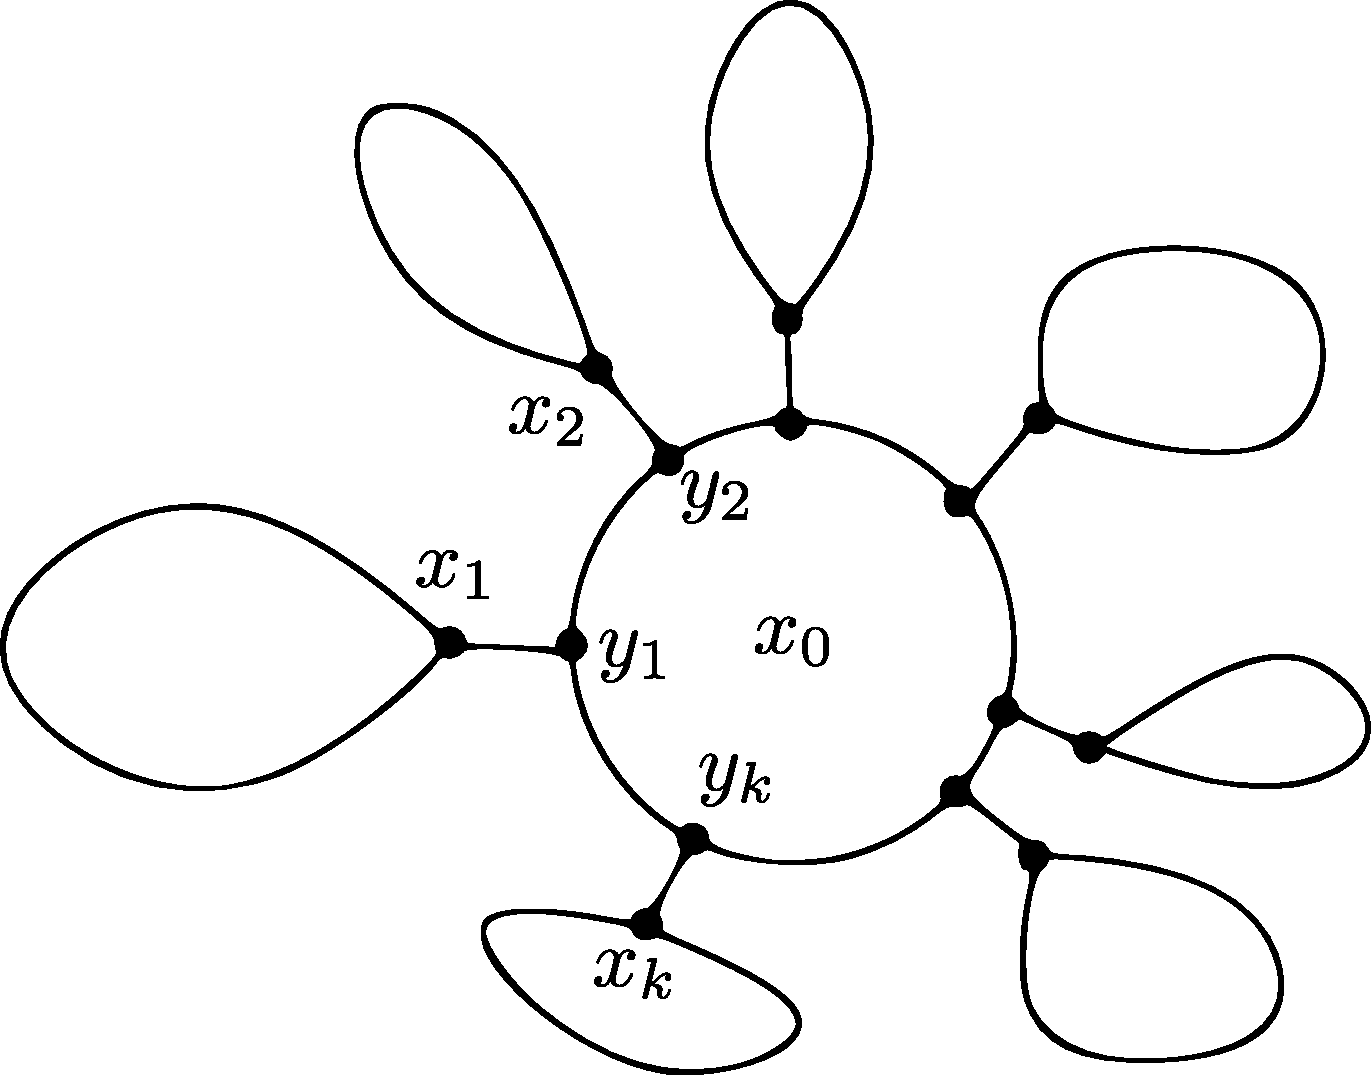
\includegraphics[width=.95\textwidth]{assets/raw/star_decomp.pdf}
  \caption{Star decomposition (reproduced from Figure 1 of~\autocite{LowerStretch05})}
  \label{fig:gtx_star_decomp}
\end{marginfigure}

Special case of graph
series parallel
\enquote{In a subsequent paper, \textcite{seriesParallel06} proved that every series-parallel
unweighted graph admits a spanning tree of average stretch $O(log n)$. This bound is tight as it
matches the lower bound established in~\autocite{cutsTrees99}.}

more special cases are in~\autocite{specialCase14}, although it's for the minimum max stretch
$t^\star$.
\enquote{Note also that a number of particular graph classes (like interval
graphs, permutation graphs, asteroidal-triple–free graphs, strongly chordal graphs,
dually chordal graphs, and others) admit tree $t$-spanners for small values of $t$}
\fi


\paragraph{Spanners}
\label{par:spanners}

As we mentioned, by stopping the \gtx{} algorithm before it finishes, we obtain a set of edges
spanning the graphs that is not a tree. Such structure are called \emph{spanner}. More precisely,
the subgraph $H$ is said to be an $t$-spanner of $G$ if, for a parameter $t \geq 1$, and for every
pair $u, v \in V$ of vertices, it holds that $d_H(u, v) \leq t \cdot d_G(u, v)$. The problem was
introduced by \textcites{SpannerFirst89}{SpannerSecond89} and has been extensively studied since
then, for it has many applications in network design. It was also showed to be \NPh{} to
approximate~\autocite{SpannerNPHard07}. The most simple construction is a greedy
algorithm~\autocite{greedySpanner93} that works similarly to the minimum spanning tree construction.
Starting from an empty subgraph $H$, it goes through every edge $(u, v)$ of $G$ sorted by weight and
check if there is a path between $u$ and $v$ in $H$ of length at most $t$. If it is case the edge
$(u,v)$ is dropped, otherwise it is inserted in $H$. This results in a $(2t - 1)$-spanner with
$O(n^{1+1/t})$ edges, which is an optimal trade-off between those two quantifies.  Furthermore on
weighted graphs, the greedy spanner total weight is essentially optimal~\autocite{GreedyOpt16}.
However, the best implementation of it, using a dynamic data structure~\autocite{fastGreedy04} is
not scalable for it runs in $O(t n^{2+\nicefrac{1}{t}})$ and cannot easily be parallelized.
Parallelization therefore requires other kind of approaches~\autocites{parSpanner08}{parSpanner15}.
Recently, \textcite{Spanner17} showed how to obtain, for any $\epsilon > 0$, a $(2t - 1)$-spanner
with $O(n^{1+1/k}/\epsilon)$ edges in $t$ rounds, with probability at least $1 - \epsilon$.

\iffalse
\url{http://www.siam.org/meetings/da17/schedule.html} SODA 13B \url{http://dl.acm.org/citation.cfm?id=3039686}
for instance the Elkin paper~\autocite{Spanner17} \enquote{Our centralized randomized algorithm computes (with
probability close to 1), a $(2k - 1)$-spanner with $n \cdot (1 + O(\frac{\log k}{n}))$ edges in
$O(|E|)$ time, whenever $k = \Omega(\log n)$. Note that when $k = \omega(\log n)$, the number of
edges is $n(1+o(1))$, i.e., in this range the algorithm computes an ultra-sparse spanner in $O(|E|)$
time.} For instance, if $k=5\log n$, we get a $10\log n$-spanner with $n\left(1+O\left(\frac{\log\log
n}{n}\right)\right)$ edges in $O(|E|)$ time.


They have applications in computing approximately shortest
paths [9, 22, 28, 37], routing [48], distance oracles and
labeling schemes [49, 56, 36] and synchronization [7].

From 6:They also appear in biology in the process of reconstructing phylogenetic trees from
matrices, whose entries represent genetic distances among contemporary living species (H. J.
Bandelt, A. W. M. Dress, Reconstructing the Shape of a Tree from Observed Dissimilarity Data, Adv.
in Appl. Math. 7 (1986)). Robotics researchers have studied spanners under the constraints of
Euclidean geometry, where vertices of the graph are points in space, and edges are line segments
joining pairs of points (Chew), (Dobkin), $[DJ], [K], [KG], [LL]$. 

studied in 1; 4; 6; 9; 15; 19; 22; 24; 26; 28; 30; 31; 37; 43; 51; 52; 57; 58



\begin{tabulary}{\textwidth}{LLLLL}
  \toprule
  work  & average stretch & edge size                              & weighted & time                                             \\
  \midrule
  46    & $4k + 1$        & $O(n^{1+\nicefrac{1}{k}})$             & no       & polynomial                                       \\
  6     & $2k +1$         & $O(n\cdot \ceil{n^{\nicefrac{1}{k}}})$ & yes      & $O\left(m(n^{1+\nicefrac{1}{k}}+n\log n)\right)$ \\
  40    & $2k-1$          & $O(n^{1+\nicefrac{1}{k}}+n)$           & no       & $O(m)$                                           \\
  Elkin & $2k-1$          & $n \cdot (1 + O(\frac{\log k}{n}))$    & no       & $O(m)$                                           \\
  \bottomrule
\end{tabulary}

% 22: E. Cohen, "Fast algorithms for constructing t-spanners and paths with stretch t," Proceedings
% of 1993 IEEE 34th Annual Foundations of Computer Science, Palo Alto, CA, 1993, pp. 648-658.  doi:
% 10.1109/SFCS.1993.366822
% We construct t-spanners of size (number of edges) Õ(n 1+(2+\epsilon)/t )
% (for any \epsilon > 0 and t such that t/(2+\epsilon) is integral). These spanners can be constructed
% by a randomized algorithm that runs in Õ(mn (2+\epsilon)/t ) time.


% Halperin and Zwick [40].  Their deterministic algorithm, for an integer parame- ter k ≥ 1,
% computes a (2k − 1)-spanner with n 1+1/k + n edges in O(|E|) time. (Their result improved previous
% pioneering work by [46, 22].)

Describe the greedy algorithm of 6. Using (55 On Dynamic Shortest Paths Problems Liam Roditty, Uri
Zwick, 2004), it runs in $O(\alpha n^{2+\nicefrac{1}{\alpha}})$

peleg 2007 hardness results

46: Peleg, D. and Schäffer, A. A. (1989), Graph spanners. J. Graph Theory, 13: 99–116.
doi:10.1002/jgt.3190130114

study the problem on unweighted graph. Application to routing scheme (48: D. Peleg and E. Upfal, A
tradeoff between space and efficiency for routing tables. 20th ACM Symposium on the Theory of
Computing, Chicago (1988))
Special case for the complete graph weighted by the distance in a 2D plan. Existing $\sqrt{10}$
spanner for the $\ell_1$ metric (L. P. Chew, There is a planar graph almost as good as the complete
graph.  Proceedings of the 2nd ACM Symposium on Computational Geometry, (1986)) (improved to
$\sqrt{4+2\sqrt{2}}$ by N. Bonichon, C. Gavoille, N. Hanusse, L. Perkovic The stretch factor of
$\ell_1$ and $\ell_{\infty}$ Delaunay triangulations European Symposium on Algorithms (ESA) (2012))
and $\phi \pi$ for $\ell_2$ (D. P. Dobkin, S. J. Friedman, and K. J. Supowit, Delaunay graphs are
almost as good as complete graphs. 28th IEEE Symposium on the Foundations of Computer Science,
(1987)) (improved to $1.998$ by Ge Xia. 2011. Improved upper bound on the stretch factor of delaunay
triangulations. In Proceedings of the twenty-seventh annual symposium on Computational geometry
(SoCG '11)). See (Prosenjit Bose, Michiel Smid, On plane geometric spanners: A survey and open
problems, Computational Geometry, Volume 46, Issue 7, 2013) for more on the 2D case.

In undirected graph, finding a spanner with less than $k$ edges is \NPc{} (theorem 2.2)
For $k<n$, one can construct in polynomial time a $(4\log_k n +1)$ spanner with less than $kn$ edges
(theorem 2.4) giving for instance ($k=2$) $O(\log n)$ spanner with $O(n)$ edges and
($k=n^{\nicefrac{1}{r}}$, $r\geq 1$) a $(4r+1)$ spanner with $O(n^{1+\nicefrac{1}{r}})$ edges
(matching lower bound within constant factor). For every $d \geq 0$, the $d$-dimensional cube has a
$3$-spanner with fewer than $7\time 2^d$ edges (Lemma 2.10 from 47: D. Peleg and J. D. Ullman. An
optimal synchronizer for the hypercube. SIAM J. on Comput., 18:740–747, 1989)
For chordal graphs: for every $n$-vertex chordal graph there exists a $2$-spanner with
$O(n\sqrt{n})$ edges (matching lower bound), a $3$-spanner with $O(n \log n)$ edges and a $5$-spanner
with $O(n)$ edges.
Much more difficult for directed graph, according to Theorem 4.2: For every $t \geq 1$ there are
infinitely many $n$-vertex directed graphs for which every $t$-spanner requires
$\Omega(\nicefrac{n^2}{t^2})$ edges.

% check some surveys of the 80's
% http://pubsonline.informs.org/doi/abs/10.1287/trsc.18.1.1
% http://onlinelibrary.wiley.com/doi/10.1002/net.3230190305/full
% early solutions
% http://onlinelibrary.wiley.com/doi/10.1002/net.3230090104/full
% http://onlinelibrary.wiley.com/doi/10.1002/net.3230130309/full
% later solution?
% http://ieeexplore.ieee.org/document/81738


While they have many applications [see first paragraph of \url{https://arxiv.org/pdf/1401.2454.pdf},
which was later merged in a STOC'14 paper] (a major one being solving linear systems), in some
practical situations their advantages are less clear [from
\url{https://link.springer.com/chapter/10.1007/978-3-319-20086-6_16}\enquote{for reasonable inputs
the constant factors make the solver much slower than methods with higher asymptotic complexity.
One other aspect predicted by theory is confirmed by our findings: Spanning trees with lower
stretch indeed reduce the solver's running time. Yet, simple spanning tree algorithms perform
better in practice than those with a guaranteed low stretch.} this is improved by
\url{https://link.springer.com/chapter/10.1007%2F978-3-319-20086-6_17} although they seem to work
	mostly with the Laplacian of the tree ]
\fi

\paragraph{Other problems}

Finding low stretch trees and spanners with respect to the existing edges is the most relevant
problem when addressing the \esp{} problem. For the sake of completeness, we nonetheless give an
overview of some related problems.

For instance, \textcite{Johnson1978} define the following problem, where the stretch is defined over
all possible pairs of nodes\footnote{We adapt their notations
to match ours}:  
\begin{problem}[Network Design Problem]
  \label{prob:gtx_ndp}
  Given an undirected integer-weighted graph $G=(V, E, w)$, a budget $B\in\Nbb$ and a criterion
  threshold $C\in \Nbb$, does there exist a spanning subgraph $G'=(V, E')$ of $G$ with weight
  $w(E') \leq B$ and criterion value $F(G') \leq C$, where the criterion function $F(G')$ denotes
  the sum of the weights of the shortest paths in $G'$ between all vertex pairs?
\end{problem}
They prove that finding such a subgraph is \NPc{}, by exhibiting a reduction from the
\textsc{Knapsack} problem. They also prove that the less general problem of finding a spanning tree
on an unweighted graph, that is
\vspace{-.5\baselineskip}
\begin{problem}[Simple Network Design Problem]
  \autoref{prob:gtx_ndp} with $w$ being the equal to $1$ for all edges in $E$ and $B=|V|-1$.
\end{problem}%
\vspace{-.5\baselineskip}
\noindent is also \NPc{} by reduction from \textsc{Exact 3-Cover}.
However, it has recently been show that this Simple Network Design problem can be approximated to a
constant factor $6$~\autocite{AllPairStrech10}. Moreover, even when the graph is weighted,
\textcite{constantDistortion07} achieve a universal constant bound for any weighted graph.

Another problem appear when the low-stretch structure $H$ can include edges not in $G$ (as long as
the distances in $H$ remain larger than the distances in $G$). This is captured by the following
problem~\autocite{OptimalNetwork69}:
\begin{problem}[Optimal Network Problem]
  \label{prob:gtx_scott}
  Given a set $V$ of $n$ vertices, find a set of spanning edges $E\subset V^2$ that minimizes
  the sum of the length of the shortest paths  between all vertex pairs while the
  total length of the resulting network does not exceed some upper bound $B\in\Nbb$.
\end{problem}
This can be seen as a special case of \autoref{prob:gtx_ndp} with $G$ being the unweighted
$n$-complete graph. \Textcite{OptimalNetwork69} proposes a backtracking solution and two local search approximate
algorithms. Some early branch and bound heuristic solutions to \autoref{prob:gtx_scott} are surveyed
in~\autocite[Section 2.3.2]{networkDesignSurvey89} although they do not come with asymptotic
guarantee on the stretch. Furthermore, \textcite{optimApproxNP80} proves that for any $\epsilon \in
(0,1)$, finding a $|V|^{1-\epsilon}$ approximation is \NPc{}.
However, if we consider the average stretches over a distribution of trees, then this approximation
factor can be reduced to $\Theta(\log n)$~\autocite{lognMetricBoundConf03}.

Finally, the stretch can also be computed for a subset of the edges. This is useful in cases where
we have prior information on the importance of individual nodes or edges.  For instance,
\textcite{RamseyTree17} show that for every $t$, any $n$-nodes graph $G=(V,E)$ has a subset $S$ of
size at least $n^{1 - \nicefrac{1}{k}}$, and a spanning tree that has stretch $O ( k \log \log n)$
between any node in $S$ and any node in $V$. Likewise, \textcite{mLAST17} describe how to maintain a
light subgraph $H$ that minimizes the distance between pairs of source and sink that are given in an
online fashion.

As shown by \autoref{tab:gtx_related_stretch}, those problems defined in the seventies are still
being discussed nowadays in top tier conferences, proving their relevance and impact beyond the
\esp{} problem.

\setlength{\fullpage}{179mm}
\begin{table}[htbp]
\begin{adjustwidth}{-2cm}{}
  \centering
  \caption{A summary of the lowest stretches achievable for various problems.
  \label{tab:gtx_related_stretch}}
  \begin{tabulary}{\fullpage}{LCCL}
    \toprule
    kind of stretch    & \multicolumn{2}{c}{only existing edges}  & extra edges allowed   \\
    \midrule
                       & tree                                     & not tree             &\\
    \cmidrule(r){2-3}
    some pairs         & $O(k\log\log n)$~\autocite{RamseyTree17} & \autocite[Section 4]{mLAST17} & --- \\
    all existing pairs & $O\left(\log n (\log\log n)\right)$~\autocite{Abraham2012}
		       & $(2t - 1)$-spanner, $O(n^{1+1/t})$ edges~\autocite{greedySpanner93}
		       & $\Theta(\log n)$ in expectation~\autocite{lognMetricBoundConf03} \\
    all possible pairs & $6$ for unweighted graphs \autocite{AllPairStrech10} and $O(1)$
                         in general \autocite{constantDistortion07}
		       & ---
		       & no need for extra edges in that case                              \\
    \bottomrule
  \end{tabulary}
\end{adjustwidth}
\end{table}
